% Standalone file -- \input{diagram} inside a figure environment in submission.tex
% Requires: tikz, amsmath (already loaded in main doc)
\usetikzlibrary{positioning, arrows.meta, fit, backgrounds}

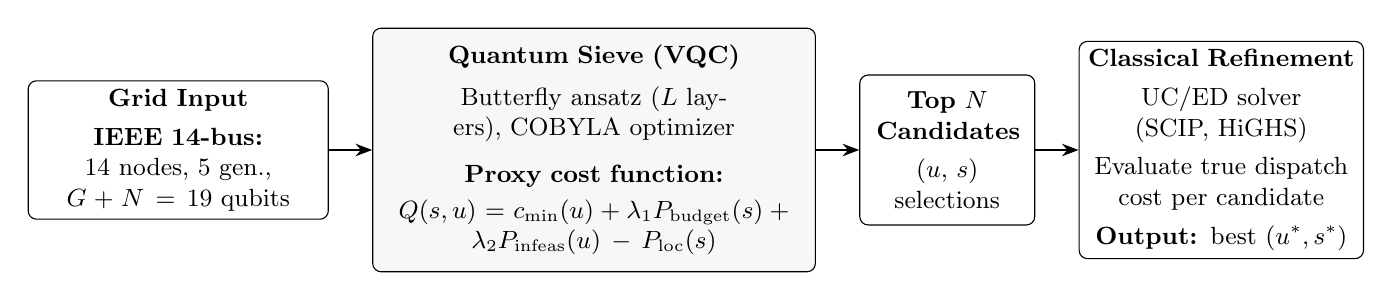
\begin{tikzpicture}[
  every node/.style={font=\small},
  box/.style={
    rectangle, draw=black, rounded corners=3pt,
    text width=#1, align=center, inner sep=6pt
  },
  arr/.style={-{Stealth[length=6pt]}, thick},
]

%% Stage 1: Grid Input
\node[box=3.6cm, inner sep=3pt] (grid) {
  \textbf{Grid Input}\\[3pt]
  \textbf{IEEE 14-bus:} 14 nodes, 5 gen., $G+N=19$ qubits\\[3pt]

};

%% Stage 2: Quantum Sieve
\node[box=5.2cm, right=0.55cm of grid, fill=gray!6] (qsieve) {
  \textbf{Quantum Sieve (VQC)}\\[4pt]
  Butterfly ansatz ($L$ layers), COBYLA optimizer\\[6pt]
  \textbf{Proxy cost function:}\\[2pt]
  $Q(s,u) = c_{\mathrm{min}}(u)
           + \lambda_1 P_{\mathrm{budget}}(s)
           + \lambda_2 P_{\mathrm{infeas}}(u)
           - P_{\mathrm{loc}}(s)$
};

%% Stage 3: Candidates
\node[box=1.8cm, right=0.55cm of qsieve] (cands) {
  \textbf{Top $N$}\\
  \textbf{Candidates}\\[3pt]
  $(u,\,s)$\\
  selections
};

%% Stage 4: Classical Refinement
\node[box=3.4cm, inner sep=3pt, right=0.55cm of cands] (classical) {
  \textbf{Classical Refinement}\\[3pt]
  UC/ED solver (SCIP, HiGHS)\\[3pt]
  Evaluate true dispatch cost per candidate\\[3pt]
  \textbf{Output:} best $(u^*,s^*)$
};

%% Arrows
\draw[arr] (grid)    -- (qsieve);
\draw[arr] (qsieve)  -- (cands);
\draw[arr] (cands)   -- (classical);

\end{tikzpicture}
